\section[Steuerungsprogramme]{Entwicklung von Steuerungsprogrammen} \label{cpt:Steuerungsprogramme}

\begin{figure}[H]
	\begin{center}
		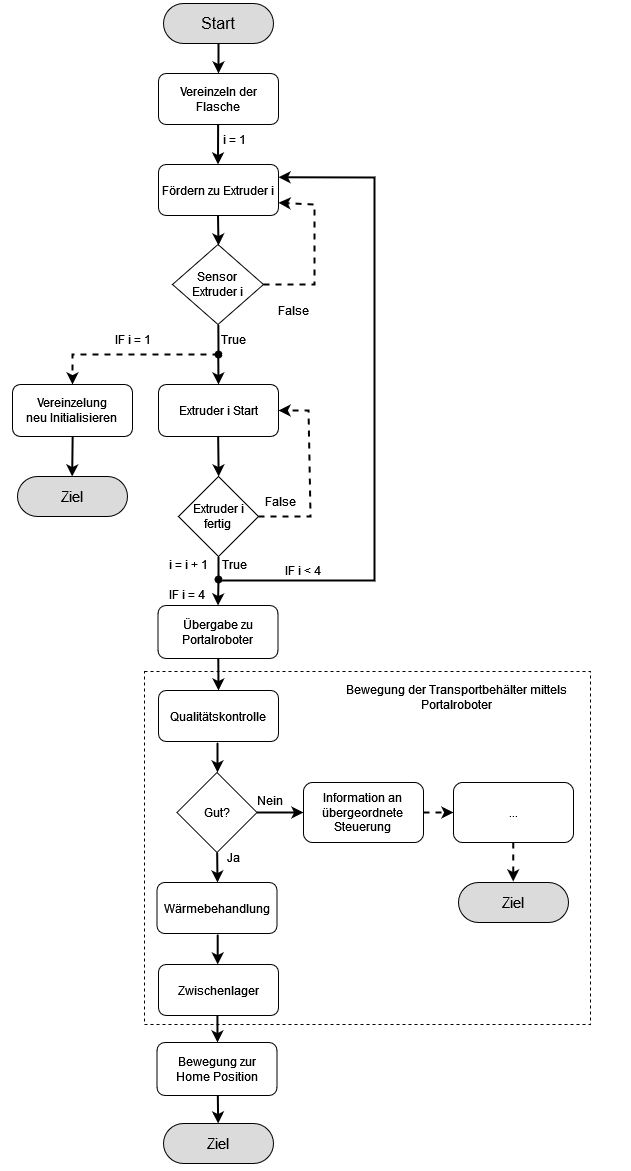
\includegraphics[width=0.8\textwidth]{images/Ablaufdiagramm.png}
		\caption{Zustandsübergangsdiagramm der Vereinzelung mit Programmierhilfen.}
		\label{fig:GesamtAblaufdiagramm}
	\end{center}	
\end{figure}

\subsection{Hierarchischer Ansatz}\label{sec:Ebenenmodell}

\begin{figure}[H]
	\begin{center}
		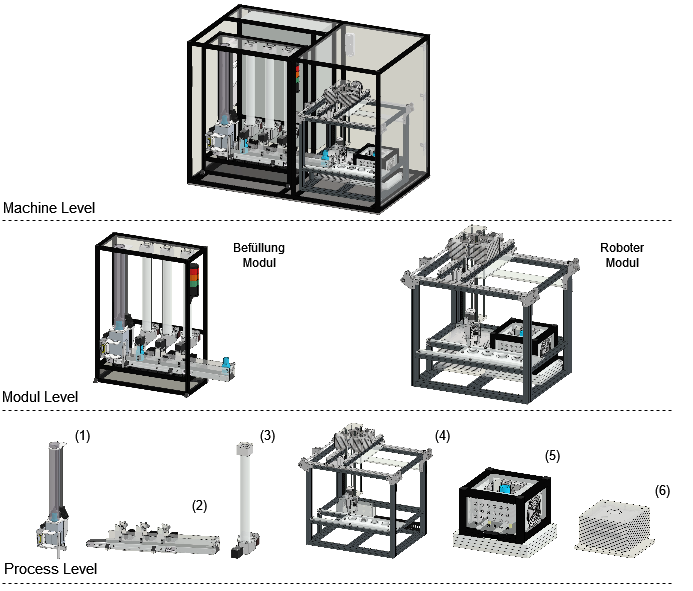
\includegraphics[width=0.7\textwidth]{images/ProgrammStruktur.png}
		\caption{Zustandsübergangsdiagramm der Vereinzelung mit Programmierhilfen.}
		\label{fig:ProgrammStruktur}
	\end{center}	
\end{figure}

\subsection{Graphengruppen}

\subsection{Übergabevariablen}

\subsection{Basisaufgaben }

\subsubsection{Abfülleinheit - 20 Punkte}

\begin{figure}[H]
	\begin{center}
		
\includegraphics[width=0.5\textwidth]{images/Schemata_Extrudermodul.png}
		\caption{O... }
		\label{fig:Schema_Extrudereinheit}
	\end{center}	
\end{figure}

\begin{figure}[H]
	\begin{center}
		
\includegraphics[width=0.6\textwidth]{images/Schemata_Abfüllmodul.png}
		\caption{O... }
		\label{fig:Schema_Abfuelleinheit}
	\end{center}	
\end{figure}

\subsubsection{Manipulatoreinheit - 20 Punkte}


\newpage
